\section{Roadmap and Timeline} \label{sec:timeline}

Table~\ref{tab:milestones} provides a list of key milestones for Rubin Operations and the Early Science Program and their nominal date ranges.
Over the course of the commissioning period, we expect these data ranges to shrink as our understanding of the remaining schedule uncertainty improves. 
% It will continue to be updated as Rubin Construction and the Early Science Program progress. 
The date ranges are derived from the Rubin ``Celebratory Milestones'', which are  published monthly on the Rubin Project website\footnote{\url{ls.st/dates}}. 

\begin{table}[ht]
\centering
\fontsize{10}{12}\selectfont 
\rowcolors{2}{white}{RubinWhite} % Alternating row colors starting at row 2
\setlength{\tabcolsep}{9pt} % Default value: 6pt
\renewcommand{\arraystretch}{1.6} % Default value: 1
\begin{tabular}[!hb]{l|l|l|l} \hline
% Table title not needed with table caption
%   \multicolumn{4}{|l|}{\textbf{Rubin Observatory Key Milestones for Early Science}} \\\hline\hline
\rowcolor{RubinTeal2} 
 \multicolumn{2}{|l|}{\textbf{Event}} &  \textbf{Notes}             &   \textbf{Date Range}  \\\hline\hline
DP0.1  & Data Preview 0.1   &  DC2 Simulated Sky Survey                &  Delivered June 2021                  \\
DP0.2 & Data Preview 0.2     &  Reprocessed DC2 Survey                 & Delivered June 2022                  \\
DP0.3 &  Data Preview 0.3     &   Solar System PPDB Simulation       & Delivered July 2023                  \\
DP1   &  Data Preview 1        &   ComCam data                                   & Oct 2024 -- Jul 2025  \\
SFL    & System First Light    &   Science-Grade Images                      & Jan 2025 -- May 2025  \\
OPS   & Start of Operations  & Operation Readiness Review  + 1 day & May 2025 -- Sep 2025 \\ 
SVY   & Start of LSST           & Rubin Operation begins + 1 day  & May 2025 -- Sep 2025 \\
DP2   & Data Preview 2        & SV Surveys complete  + 6 months  &  Nov 2025 -- May 2026 \\
DR1   & Data Release 1        & LSST  first 6 months data & May 2026 -- Jan 2027 \\
DR2   & Data Release 2        & LSST  year 1 data & May 2027 -- Jan 2028 \\
DR3   & Data Release 3        & LSST  year 2 data &  May 2028 -- Nov 2028 \\\hline\hline
\end{tabular}
\caption{Rubin Operations Key Milestones for Early Science}
\label{tab:milestones}
\end{table}


Milestone dates are given as min -- max ranges to indicate the associated uncertainty. 
Typically the near date corresponds to the current Project forecast, plus any additional operational uncertainty.
The late date corresponds approximately to the current Project ``late date'' plus any additional operational uncertainty.
An intermediate (typically mid-range) date is used by the Rubin Operations teams for planning purposes. 

The next key milestone in the Early Science Program is the release of DP1.
The LSST start is currently expected to be sometime between May 2025 and September 2025.
The timing of the Commissioning observations their release to the community can only be projected to within a few months at the time of writing.
The late dates for the DP2 and DR1 milestones allow for the possibility that the Project completes within its late date, but in doing so spends less time on-sky with LSSTCam.
In this eventuality, the operations team would spend up to 2 months prior to commencing the 10-year LSST survey collecting more on-sky data to complement and extend the datasets collected during commissioning (see \S~\ref{ssec:scenarios}. 

%Table \ref{tab:timeline} shows the nominal date ranges for the various elements of the Early Science Program. 
%The shaded region contains roughly 80\% of the probability, while the lefthand edge of the shaded range indicates the earliest date the milestone could be reached. 
%The darker regions give a very rough indication of the +/-1 sigma error bars. 
%Over the course of the commissioning period, we expect these shaded regions to shrink as our understanding of the remaining schedule uncertainty improves. 
%However, there is still the possibility of the assumptions underlying these distributions being wrong: this is just our best estimate at the current time.

%
%\begin{table}[ht]
%\centering
%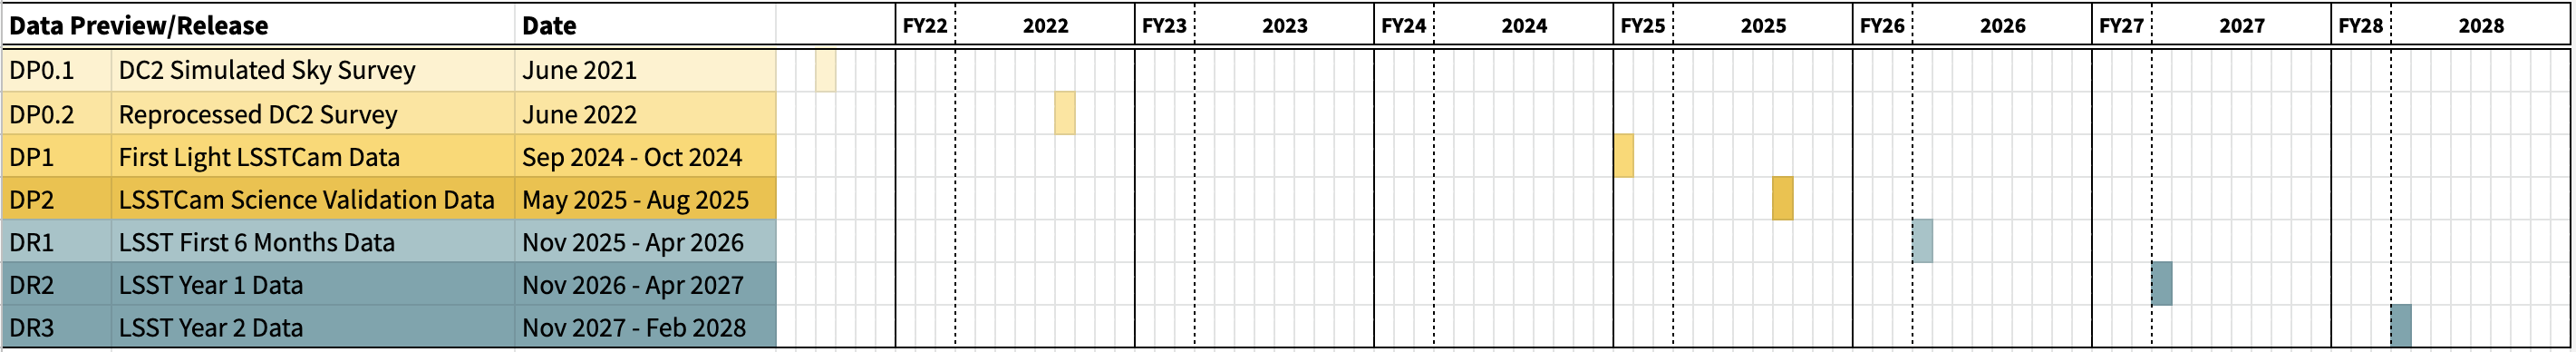
\includegraphics[width=\linewidth]{figures/DPR-timeline}
%\caption{Nominal date ranges for the various elements of the Early Science Program.}
%\label{tab:timeline}
%\end{table}

Table ~\ref{tab:milestones} will continue to be refined and updated in future version of this document as the Early Science Program progresses.
